\section{Maximal Cliques and MPQ-trees} \label{sec:maximal_cliques}

In this section, we review well-known properties of interval graphs. First, we describe their
characterization in terms of orderings of maximal cliques. Then, we introduce two data structures to
deal with these orderings, namely, PQ-trees and MPQ-trees. Finally, we prove some simple structural
results concerning MPQ-trees.

\heading{Consecutive Orderings.}
Fulkerson and Gross~\cite{maximal_cliques} proved the following fundamental characterization of interval
graphs:

\begin{figure}[b!]
\centering
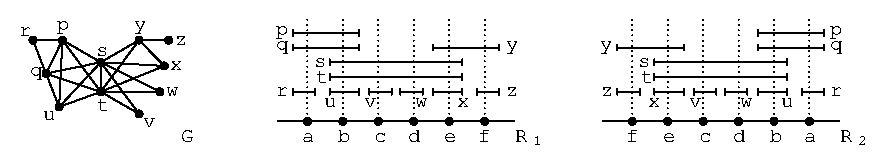
\includegraphics{maximal_cliques_fulkerson_gross.eps}
\caption{An interval graph $G$ and two of its representations with different left-to-right orderings
$<$ of the maximal cliques. Some choices of clique-points are depicted on the real lines.}
\label{fig:fulkerson_gross}
\end{figure}

\begin{figure}[b!]
\centering
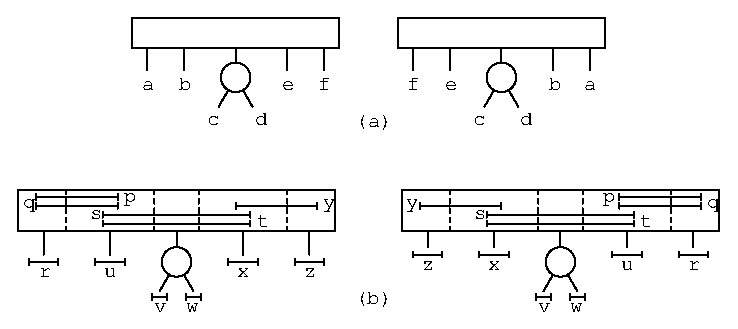
\includegraphics{maximal_cliques_pq_trees.eps}
\caption{(a) Two equivalent PQ-trees with frontiers $a < b < c < d < e < f$ and $f < e < c < d < b <
a$, respectively. In all figures, we denote P-nodes by circles and Q-nodes by rectangles. (b)~The
corresponding MPQ-trees with depicted sections.}
\label{fig:pq_trees}
\end{figure}

\begin{lemma}[Fulkerson and Gross~\cite{maximal_cliques}] \label{lem:maximal_cliques}
A graph is an interval graph if and only if there exists a linear ordering $<$ of its maximal
cliques such that, for each vertex, the maximal cliques containing this vertex appear consecutively.
\end{lemma}

We call an ordering of the maximal cliques satisfying the statement of
Lemma~\ref{lem:maximal_cliques} a \emph{consecutive ordering}. See Fig.~\ref{fig:fulkerson_gross}
for an example. The ordering $<$ from the statement is obtained by sweeping an interval
representation from left to right. By the Helly property, the intervals of every maximal clique have
a non-empty intersection. For all maximal cliques, these intersections are disjoint and ordered from
left to right. In the intersection of the intervals of a maximal clique $a$, we pick one point which
we call a \emph{clique-point} $\cp(a)$. The left-to-right ordering of these clique-points gives $<$.
On the other hand, given a consecutive ordering $<$, we place the clique-points from left to right
according to $<$ and construct an interval representation by placing each interval on top of its
clique-points and no others. This can be done because the ordering places the maximal cliques
containing each of the vertices consecutively.

\heading{PQ-trees.} Booth and Lueker~\cite{PQ_trees} designed a data structure called PQ-trees to
efficiently work with consecutive orderings of maximal cliques. A \emph{PQ-tree} $T$ is a rooted
tree. Its leaves are in one-to-one correspondence with the maximal cliques. Its inner nodes are of
two types: \emph{P-nodes} and \emph{Q-nodes}. Each P-node has at least two children, and each Q-node
has at least three. Further, for every inner node, a left-to-right ordering of its children is
given. Every PQ-tree $T$ represents one linear ordering $<_T$ of the maximal cliques called the
\emph{frontier} of $T$, which is the ordering of the leaves from left to right.

Every PQ-tree $T$ further represents other linear orderings. These orderings are frontiers of
equivalent PQ-trees. A PQ-tree $T'$ is \emph{equivalent} to $T$ if it can be constructed from $T$ by
a sequence of \emph{equivalent transformations} of two types: (i) an arbitrary reordering of the
children of a P-node, and (ii) a reversal of the order of the children of a Q-node.
Fig.~\ref{fig:pq_trees}a depicts two equivalent PQ-trees corresponding to the interval graph from
Fig.~\ref{fig:fulkerson_gross}.

Booth and Lueker proved that, for every interval graph, there exists a unique PQ-tree (up to
equivalence transformations) representing precisely the consecutive orderings of the maximal
cliques. In other words, this tree describes all possible interval representations of this interval
graph. 

A subtree of $T$ consists of a node and all its descendants. The subtrees of a node $N$ are those
subtrees having the children of $N$ as the roots. For a node $N$, let $T[N]$ denote the subtree of
$T$ with the root $N$.

\heading{MPQ-trees.}
For the purpose of this paper, we need more information about the way in which the vertices of the
interval graph are related to the structure of the PQ-tree. This additional information is contained
in the \emph{modified PQ-tree} (MPQ-tree), introduced by Korte and M\"ohring~\cite{korte_mohring}.
We note that the same idea is already present in the earlier paper of Colbourn and
Booth~\cite{colbourn_booth}.

The MPQ-tree is an augmentation of the PQ-tree in which the nodes of $T$ have assigned subsets of
$V(G)$ called \emph{sections}.  To a leaf representing a clique $a$, we assign one section $s(a)$.
Similarly, to each P-node $P$, we assign one section $s(P)$. For a Q-node $Q$ with $n$ children,
we have $n$ sections $s_1(Q),\dots,s_n(Q)$, each corresponding to one subtree of $Q$.

The section $s(a)$ has all vertices contained in the maximal clique $a$ and no other maximal clique.
The section $s(P)$ of a P-node $P$ has all vertices that are contained in all maximal cliques of
$T[P]$ and in no other maximal clique. Sections of Q-nodes are more complicated.
Let $Q$ be a Q-node with subtrees $T_1,\dots,T_n$. Let $x$ be a vertex contained only in maximal
cliques of $T[Q]$, and suppose that it is contained in maximal cliques of at
least two subtrees. Then $x$ is contained in every section $s_i(Q)$ such that some maximal clique of
$T_i$ contains $x$. Fig.~\ref{fig:pq_trees}b depicts the sections for the example in
Fig.~\ref{fig:fulkerson_gross}.

Korte and M\"ohring~\cite{korte_mohring} state the following properties:
\begin{packed_itemize}
\item Every vertex $x$ is placed in the sections of exactly one node of $T$. In the case of a
Q-node, it is placed in consecutive sections of this node.
\item For a Q-node $Q$, if $x$ is placed in a section $s_i(Q)$, then $x$ is contained in all cliques
of $T_i$.
\item Every section of a Q-node is non-empty. Moreover, two consecutive sections have a non-empty
intersection.
\item A maximal clique contains exactly those vertices contained in the sections encountered when we traverse the
tree from the corresponding leaf to the root.
\end{packed_itemize}

\heading{Structure of MPQ-trees.} Next, we show several structural properties used in
building minimal obstructions which are quite easy to prove:

\begin{lemma} \label{lem:different_sections}
Let $Q$ be a Q-node. Then $s_i(Q) \ne s_j(Q)$ for every $i \ne j$. Further, if $s_i(Q) \subsetneq
s_{i+1}(Q)$, then at least one section of $T_i$ is non-empty. 
\end{lemma}

\begin{proof}
If $s_i(Q) = s_j(Q)$, then we could exchange $T_i$ and $T_j$ and we would obtain a valid MPQ-tree
for $G$. Since $n \ge 3$, this yields a contradiction with the fact that the only possible
transformation of a $Q$-node is reverting the order of its children.

For the latter part, let $a$ and $b$ respectively be maximal cliques of a leaf in $T_i$ and a leaf in $T_{i+1}$. Then $a \setminus b \neq \emptyset$ and
every $x \in a \setminus b$ belongs to sections of $T_i$.\qed
\end{proof}

Let $N$ be a node of the MPQ-tree. By $G[N]$ we denote the subgraph induced by all the
vertices in the sections of the subtree rooted at $N$. Similarly, for a subtree $T'$, we denote the
subgraph induced by the vertices in its sections by $G[T']$.

\begin{lemma} \label{lem:connectivness}
Let $N$ be an inner node of an MPQ-tree.
\begin{packed_itemize}
\item[(i)] If $N$ is a Q-node, then $G[N]$ is connected.
\item[(ii)] If $N$ is a P-node, then $G[N]$ is connected if and only if $s(N)$ is non-empty.
Furthermore, for every child $T_i$ of $N$, the graph $G[T_i]$ is connected.
\end{packed_itemize}
\end{lemma}

\begin{proof}
(i)
%For a Q-node, if $G[N]$ is not connected, we can swap the components arbitrarily.  Since $N$ has at
%least three children, this would contradict only two possible orderings of the subtrees.
%Alternatively,
It follows from the facts that the vertices in any section form a clique, and that
any two consecutive sections of $N$ have non-empty intersection.

(ii) The first statement is clear. For the second part, notice that if $G[T_i]$ was not connected, we
could permute the connected components of $G[T_i]$ arbitrarily with the other children of $N$.  Therefore
$T_i$ would not be a child of $N$, but $N$ would have one child per each connected component of
$G[T_i]$.\qed
\end{proof}

Let $Q$ be a Q-node and $i < j$. Let $x$ and $y$ be two vertices of $G[Q]$, where $x$ is either
in $T_i$, or $s_i(Q)$, and $y$ is either in $T_j$, or $s_j(Q)$. A path $P_{x,y}$ is called
\emph{$Q$-monotone} if all inner vertices of the path belong to the sections of $Q$, and their
leftmost/rightmost sections strictly increase.

\begin{lemma} \label{lem:monotone_paths}
Let $H$ be an induced subgraph of $G[Q]$ such that $x,y \in V(H)$ belong to one component.
Then every shortest path $P_{x,y}$ in $H$ is $Q$-monotone.
\end{lemma}

\begin{proof}
It is easy to see that any path from $x$ to $y$ that is not $Q$-monotone can be shortened.\qed
\end{proof}

Let $Q$ be a Q-node. Let $u$ be a vertex appearing in sections of $T[Q]$. If $u$ belongs to sections
of $Q$, let $s_u^\lft(Q)$ be the leftmost section of $Q$ containing $u$ and $s_u^\rt(Q)$ be the
rightmost one. If $u$ belongs to sections of a subtree $T_i$ of $Q$, we put $s_u^\lft(Q) =
s_u^\rt(Q) = s_i(Q)$.  If $s_u^\rt(Q)$ is on the left of $s_v^\lft(Q)$, then we say that \emph{$u$
is on the left of $v$} and \emph{$v$ is on the right of $u$}. Also, \emph{$u$ and $v$ are on the
same side of $w$} if they are both on the left of $w$, or both on the right of $w$. Similarly,
\emph{$v$ is between $u$ and $w$} if either $u$ is on the left and $w$ is on the right of $v$, or
$u$ is on the right and $w$ is on the left of $v$. For a maximal clique $a \in T_i$, we
say that \emph{$u$ is on the left of $a$} when $s_u^\rt(Q)$ is on the left of $s_i(Q)$, and
similarly the other relations.

\heading{Non-adjacencies of Maximal Cliques.} Maximal cliques of interval
graphs have the following special property, which we use to build minimal obstructions.

\begin{lemma} \label{lem:non_adjacent}
Let $H$ be a connected subgraph of an interval graph and let $c$ be a maximal clique with no vertex
in $V(H)$. There exists $x \in c$ non-adjacent to all vertices of $V(H)$.
\end{lemma}

\begin{proof}
Consider an interval representation $\calR$. It places all intervals of $H$ to one side of
$\cp(c)$, say on the left. Let $x$ be the interval of $c$ having the rightmost left endpoint. If $x$
is adjacent to some vertex $y \in V(H)$, then every vertex of $c$ is adjacent to $y$.  Since $c$ is
maximal, it follows that $y \in c$, contradicting the assumption. So $x$ is non-adjacent to all
vertices of $V(H)$.\qed
\end{proof}

